\chapter{Implementasi dan Pengujian}
Pada bagian ini akan dijelaskan tentang implementasi dan pengujian yang
dilakukan. Implementasi adalah tahapan setelah proses perancangan selesai,
rancangan yang sudah dibuat, diimplementasikan menggunakan kode program. Bahasa
pemrograman yang digunakan adalah javascript. Setelah implementasi dilakukan,
akan dilakukan juga beberapa pengujian. Pengujian dilakukan untuk mengetahui
apakah fungsi-fungsi utama aplikasi sudah berjalan dengan baik dan
juga untuk mengetahui kekurangan yang dimiliki aplikasi tersebut.

\section{Implementasi}
Implementasi dilakukan menggunakan bahasa pemrograman javascript, hasil
implementasi adalah dokumen HTML. Berikut ini adalah beberapa bagian dari hasil
implementasi, keseluruhan hasil implementasi dapat dilihat pada Lampiran A:
\begin{itemize}
  \item Pembuatan Kelas Node dan Kelas Neighbor \\
  Berikut ini adalah hasil implementasi dalam bentuk kode program dari kelas
  node dan neighbor. Kedua kelas tersebut merupakan komponen utama untuk
  pembuatan graf.
\lstset{basicstyle=\scriptsize}
\begin{lstlisting}
//Kelas Node
function Node(id, neighbors){
  this.id = id;
  this.adjList = neighbors;
}

//Kelas Neighbor
function Neighbor(vnum, nbr, weight){
  this.vertexNum = vnum;
  this.next = nbr;
  this.weight = weight;
}
\end{lstlisting}
  
  \item Pemodelan OSMXML menjadi graf. \\
  Berikut ini adalah hasil implementasi dalam bentuk kode program yang berfungsi
  untuk memodelkan OSMXML menjadi graf
\begin{lstlisting}
for(v=0; v < node.length; v++){
  adjLists.push(new Node(node[v].getAttribute('id'),null));
}

for (i=0;i<way.length;i++){
  nd = way[i].getElementsByTagName("nd");
  if(isHighway(way,i)){
    oneway = wayDirection(way,i);
    for (j=0;j<nd.length-1;j++){
      //cari jarak 
      v1 = indexForId(adjLists,nd[j].getAttribute('ref'));
      v2 = indexForId(adjLists,nd[j+1].getAttribute('ref'));	
      lat1 = getLatByAtt(nd[j].getAttribute('ref'));
      lon1 = getLonByAtt(nd[j].getAttribute('ref'));
      lat2 = getLatByAtt(nd[j+1].getAttribute('ref'));
      lon2 = getLonByAtt(nd[j+1].getAttribute('ref'));
      
      point1 = new google.maps.LatLng(lat1,lon1);
      point2 = new google.maps.LatLng(lat2,lon2);
      distance = google.maps.geometry.spherical.
      computeDistanceBetween(point1,point2);
	  
      //memasukkan informasi edge		
      if(oneway == "yes"){
        adjLists[v1].adjList = new Neighbor(v2,
        adjLists[v1].adjList,distance); 
      }else if(oneway == "no"){
        adjLists[v1].adjList = new Neighbor(v2,
        adjLists[v1].adjList,distance); 
        adjLists[v2].adjList = new Neighbor(v1,
        adjLists[v2].adjList,distance);
      }else if(oneway == "-1"){
        adjLists[v2].adjList = new Neighbor(v1,
        adjLists[v2].adjList,distance); 
      }else{
        adjLists[v1].adjList = new Neighbor(v2,
        adjLists[v1].adjList,distance); 
        adjLists[v2].adjList = new Neighbor(v1,
        adjLists[v2].adjList,distance); 
      }	
    }
  }
}
\end{lstlisting}

  \item Visualisasi Graf \\
  Berikut ini adalah hasil implementasi kode program yang berfungsi untuk
  menampilkan node dan edge pada peta dijital.
\begin{lstlisting}
this.generate = function(){
		for (i=0;i<way.length;i++)
		{
			nd = way[i].getElementsByTagName("nd");
			if(isHighway(way,i))
			{
				for (j=0;j<nd.length;j++)
				{
					id = uniqueId();
					marker = new google.maps.Marker({
						id: id,
						position: new google.maps.LatLng(getLatByAtt(nd[j].getAttribute('ref')), getLonByAtt(nd[j].getAttribute('ref'))),
						map: map,
						icon: image,
					});
					markers[id] = marker;

					content = 'Id Node : '+nd[j].getAttribute('ref')+'<br>'+
					'Index Node : '+indexForId(list,nd[j].getAttribute('ref'))+'<br>'+
					'<a href="#" onclick="setAsal(\'' + id + '\',\'' + nd[j].getAttribute('ref') + '\',\'' + indexForId(list,nd[j].getAttribute('ref')) + '\')">Pilih sebagai asal</a>'+'<br>'+
					'<a href="#" onclick="setTujuan(\'' + id + '\',\'' + nd[j].getAttribute('ref') + '\',\'' + indexForId(list,nd[j].getAttribute('ref')) + '\')">Pilih sebagai tujuan</a>';
					
					addInfoWindow(marker, content);	
				}
				
				for (k=0;k<nd.length-1;k++)
				{
					line = new google.maps.Polyline({
						path: [new google.maps.LatLng(getLatByAtt(nd[k].getAttribute('ref')), getLonByAtt(nd[k].getAttribute('ref'))),
						new google.maps.LatLng(getLatByAtt(nd[k+1].getAttribute('ref')), getLonByAtt(nd[k+1].getAttribute('ref')))],
						strokeColor: "#000000",
						strokeOpacity: 1,
						strokeWeight: 3,
						map: map
					});
				}
			}
		}
		return markers;
	}
\end{lstlisting}

  \item Pencarian Rute Terdekat \\
  Berikut ini adalah hasil implementasi algoritma Dijkstra untuk pencarian rute
  terdekat.
\begin{lstlisting}
this.shortestPath = function(asal, tujuan){
	var PQ = new PriorityQueue();
	var	distances = {};
	var	previous = {};
	var	path = [];
	var	smallest, node, neighbor, alt;
		
	for(node in this.nodes){
		if(node === asal){
			distances[node] = 0;
			PQ.enqueue(0, node);
		}
		else{
			distances[node] = INFINITY;
			PQ.enqueue(INFINITY, node);
		}
		previous[node] = null;
	}
		
	while(!PQ.isEmpty()){
		try{
			smallest = PQ.dequeue().key;
			if(smallest === tujuan){
				while(previous[smallest]){
					path.push(smallest);
					smallest = previous[smallest];
				}
				break;
			}
				
			if(distances[smallest] === INFINITY){
				break;
			}

			for(neighbor in this.nodes[smallest]){
				alt = distances[smallest] + this.nodes[smallest][neighbor];
				if(alt < distances[neighbor]) {
					distances[neighbor] = alt;
					previous[neighbor] = smallest;
					PQ.enqueue(alt, neighbor);
				}
			}
		}catch(err){
			return path;
		}
	}
	return path;
}
\end{lstlisting}
\end{itemize}

\section{Pengujian}
Pada subbab ini dibahas lingkungan pengujian dan pengujian yang dilakukan.
Pengujian yang dilakukan dibagi menjadi dua tahap yaitu pengujian fungsional 
dan pengujian eksperimental.
Pengujian fungsional menguji tampilan antar muka aplikasi beserta method atau
fungsi dasar, sedangkan pengujian eksperimental dilakukan dengan menggunakan
tiga dokumen OSMXML yang berbeda.

\subsection{Lingkungan Pengujian}
Berikut ini adalah lingkungan pengujian aplikasi:
\begin{enumerate}
  \item Processor\\
  Intel Core i5-2410M CPU @ 2.30Ghz (4 CPU)
  
  \item Memory\\
  4096MB RAM
  
  \item Display\\
  AMD Radeon HD 6470M
  
  \item Operating System\\
  Windows 7 Ultimate 64-bit
  
  \item Browser\\
  Google Chrome Version 41.0.2272.118 m 
\end{enumerate}

\subsection{Pengujian Fungsional}
Pengujian fungsional menguji tampilan antar muka aplikasi beserta method atau
fungsi dasar. Seluruh pengujian fungsional menggunakan OSMXML
yang bernama ``bandung1.xml'', batas area pada dokumen ini memiliki batas
koordinat yaitu <bounds minlat="-6.9076500" minlon="107.5961800" maxlat="-6.9044500" 
maxlon="107.6016300"/>, cakupan area tersebut berlokasi di Kota Bandung. Untuk
dokumen bandung1.xml dapat dilihat pada Lampiran B. Berikut ini adalah daftar
fungsi yang diujikan:
\begin{enumerate}
  \item Tampilan antar muka.\\
  Pada tampilan antar muka aplikasi terdapat elemen ``<div>'' sebagai tempat
  untuk menampilkan peta dengan ukuran lebar 75\% dari lebar layar dan tinggi 600px. 
  Di sebelah kanan layar terdapat 2 buah \textit{TextBox} yang menampilkan informasi titik asal
  dan titik tujuan ketika \textit{user} memilih. Selain itu, terdapat 2 buah
  tombol yaitu ``Cari!'' untuk mencari rute terdekat antara kedua titik
  dan tombol kedua adalah ``Reload'' untuk memuat ulang aplikasi. Hasil
  pengujian tampilan antar muka dapat dilihat pada Gambar \ref{fig:pu_antarmuka}.
\begin{figure}[h]
\centering
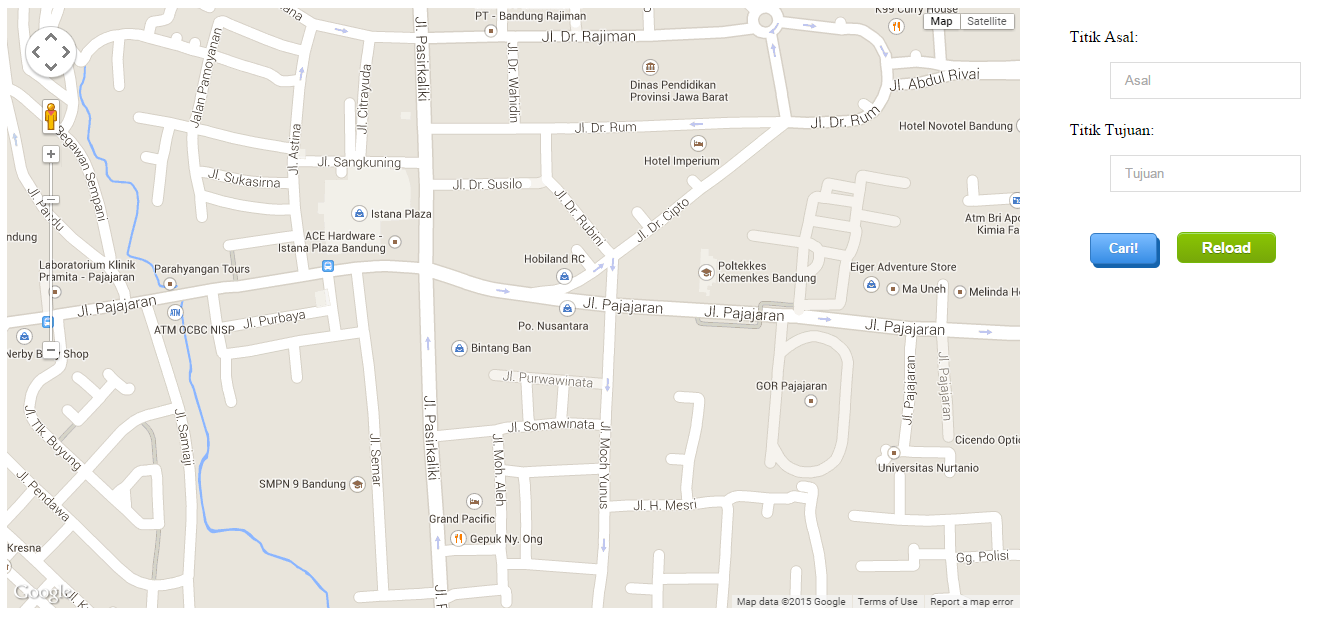
\includegraphics[scale=0.45]{Gambar/pu_antarmuka}
\caption[Pengujian Antar Muka]{Pengujian Antar Muka}
\label{fig:pu_antarmuka}
\end{figure}
  
  \item Fungsi untuk membaca dokumen OSMXML.\\
  Aplikasi mendapatkan informasi dari dokumen OSMXML. Pengujian
  fungsi ini dilakukan untuk memastikan bahwa dokumen OSMXML dapat dibaca dengan
  baik. Pengujian dilakukan dengan cara membandingkan dokumen OSMXML dengan
  informasi yang sudah dibaca. Contoh kasus adalah membandingkan 10 node
  pertama, potongan informasi 10 node pertama pada ``test.xml'' dapat dilihat
  pada Gambar \ref{fig:pu_osmxml2} dan hasil pengujian dapat dilihat pada Gambar
  \ref{fig:pu_osmxml1}. Pada Gambar \ref{fig:pu_osmxml2} menunjukkan bahwa hasil
  pembacaan sama dengan ``test.xml'' pada Gambar \ref{fig:pu_osmxml1}, hal ini
  menunjukkan fungsi untuk membaca dokumen OSMXML sudah berjalan dengan baik.
\begin{figure}[h]
\centering
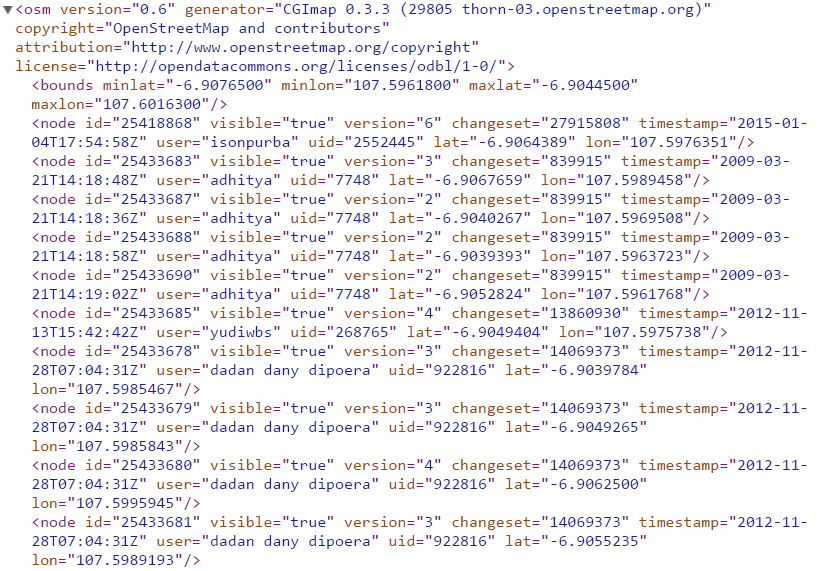
\includegraphics[scale=0.7]{Gambar/pu_osmxml2}
\caption[Dokumen test.xml]{Dokumen bandung1.xml}
\label{fig:pu_osmxml2}
\end{figure}

\begin{figure}[h]
\centering
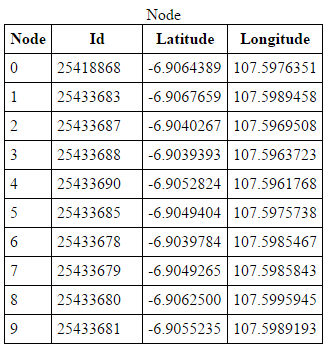
\includegraphics[scale=1]{Gambar/pu_osmxml1}
\caption[Pengujian Fungsi OSMXML]{Pengujian Fungsi OSMXML}
\label{fig:pu_osmxml1}
\end{figure}
\clearpage

  \item Fungsi untuk mengukur jarak antara dua titik.\\
  Pengukuran jarak antara dua titik menggunakan \textit{geometry spherical}.
  Contoh kasus adalah mencari jarak setiap titik yang terdapat pada tag way
  dengan id 190605660, hasil pengujian dapat dilihat pada Gambar
  \ref{fig:pu_jarak1} dan \ref{fig:pu_jarak2}.
\begin{figure}[h]
\centering
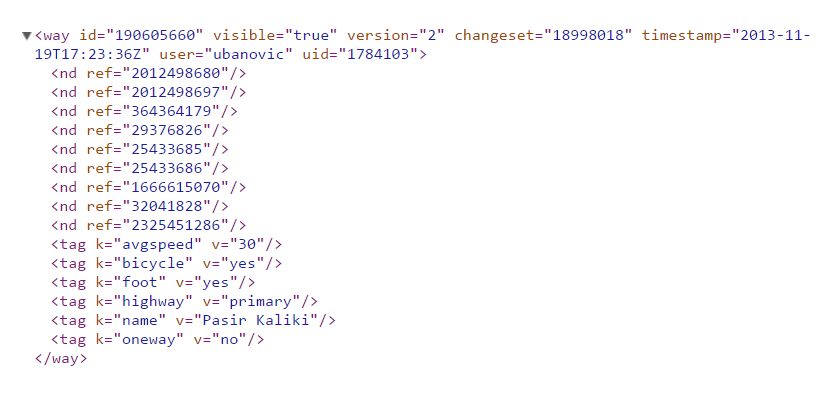
\includegraphics[scale=0.7]{Gambar/pu_jarak1}
\caption[Dokumen test.xml]{Dokumen bandung1.xml}
\label{fig:pu_jarak1}
\end{figure}

\begin{figure}[h]
\centering
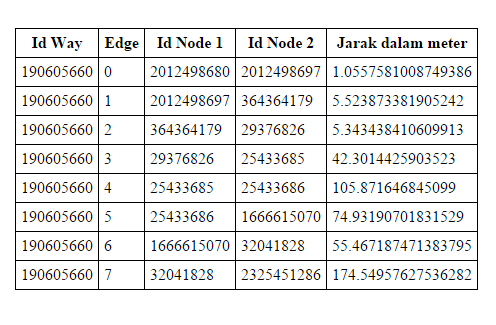
\includegraphics[scale=1]{Gambar/pu_jarak2}
\caption[Pengujian Jarak]{Pengujian Jarak}
\label{fig:pu_jarak2}
\end{figure}

\item Fungsi untuk mengubah informasi OSMXML menjadi graf.
\begin{figure}[h]
\centering
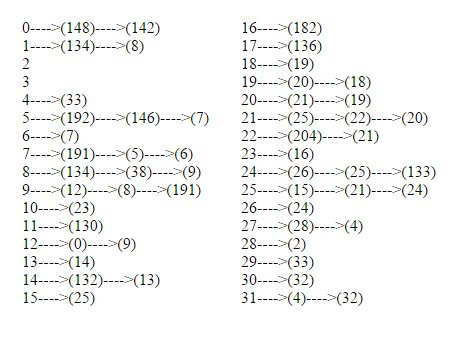
\includegraphics[scale=1]{Gambar/pu_graf}
\caption[Pengujian Fungsi OSMXML Menjadi Graf]{Pengujian Fungsi OSMXML Menjadi Graf}
\label{fig:pu_graf}
\end{figure}\\
  Informasi yang didapatkan dari OSMXML, selanjutnya diubah menjadi graf.
  Pengujian dilakukan dengan mengubah seluruh ``test.xml'' menjadi graf
  menggunakan \textit{adjacency list}. Berikut hasil pengujian, dapat dilihat
  pada Gambar \ref{fig:pu_graf}. Pada Gambar \ref{fig:pu_graf} hanya ditampilkan
  hingga 32 node, hal ini dikarenakan ``bandung1.xml'' memiliki 125 buah node
  dan terlalu banyak jika ditampilkan seluruhnya.
  
  \item Fungsi untuk melakukan visualisasi.\\
  Fungsi ini menggambarkan setiap node menggunakan \textit{marker} dan
  setiap edge menggunakan \text{polyline} pada peta, hasil pengujian dapat
  dilihat pada Gambar \ref{fig:pu_visual}.
\begin{figure}[h]
\centering
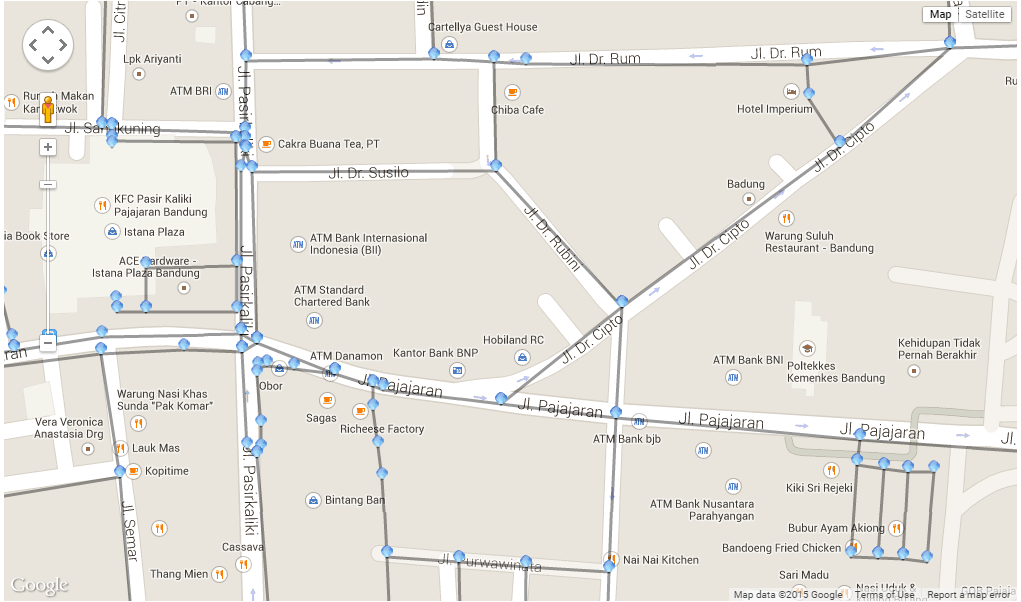
\includegraphics[scale=0.48]{Gambar/pu_visual}
\caption[Pengujian Fungsi Visualisasi]{Pengujian Fungsi Visualisasi}
\label{fig:pu_visual}
\end{figure}

  \item Fungsi untuk memilih titik asal dan titik tujuan.\\
  Pengujian dilakukan dengan memilih titik asal dan titik tujuan. Titik asal
  yang sudah dipilih berganti \textit{icon} dengan warna hijau dan titik tujuan
  yang sudah dipilih berganti \textit{icon} dengan warna merah. Informasi
  Id Node dari kedua titik yang sudah dipilih, ditampilkan di sebelah kanan
  layar. Hasil pengujian dapat dilihat pada Gambar \ref{fig:pu_titik}.
\begin{figure}[h]
\centering
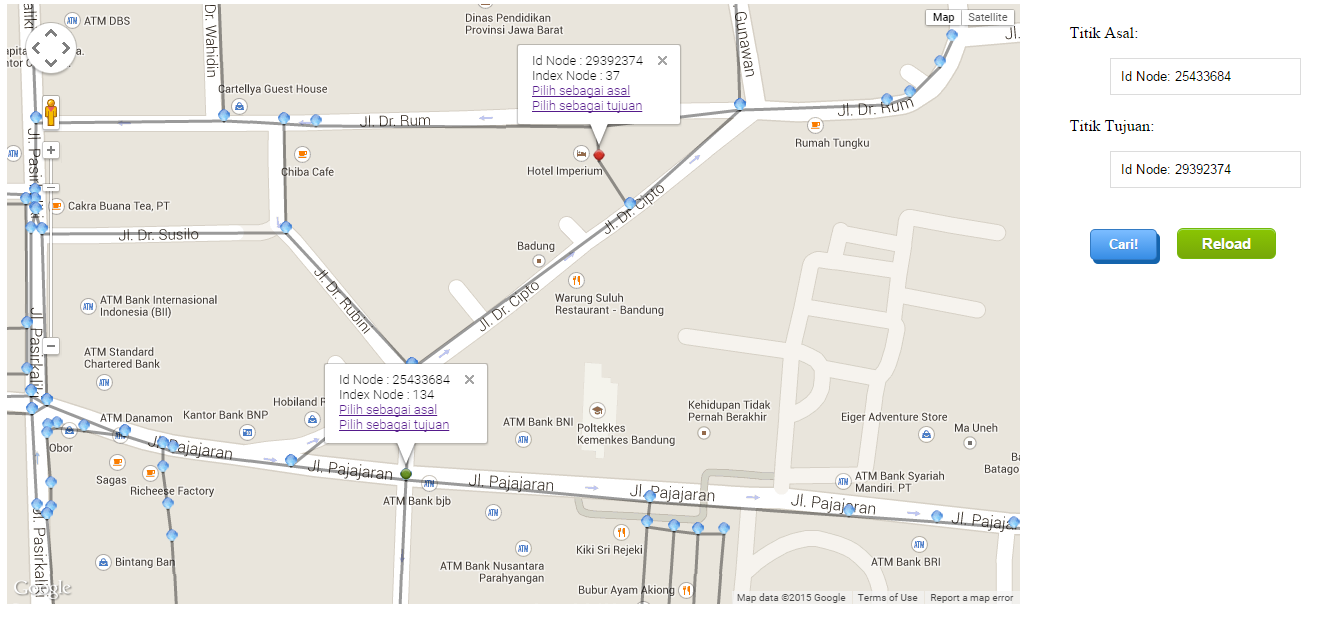
\includegraphics[scale=0.45]{Gambar/pu_titik}
\caption[Pengujian Titik Asal dan Tujuan]{Pengujian Titik Asal dan Tujuan}
\label{fig:pu_titik}
\end{figure}
  
  \item Fungsi untuk mencari rute terdekat antar dua titik menggunakan
  algoritma dijkstra.\\
  Pengujian dilakukan dengan contoh kasus mencari rute terdekat dari titik asal
  (id node : 29356381, index node : 16) ke titik tujuan (id node : 25500626,
  index node : 11), hasil pengujian dapat dilihat pada Gambar \ref{fig:pu_rute}.
\begin{figure}[h]
\centering
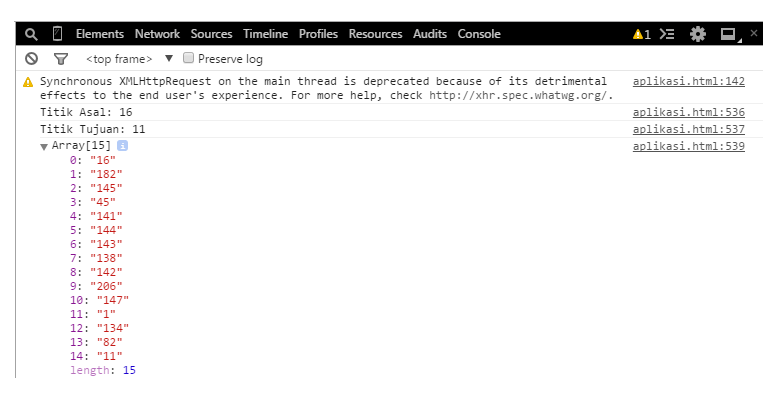
\includegraphics[scale=0.8]{Gambar/pu_rute}
\caption[Pengujian Rute Terdekat]{Pengujian Rute Terdekat}
\label{fig:pu_rute}
\end{figure}

  \item Fungsi untuk visualisasi rute terdekat.\\
  Pengujian dilakukan dengan contoh kasus yang sama pada fungsi pencari rute
  terdekat, rute terdekat digambarkan dengan \textit{polyline} berwarna
  merah. Hasil pengujian dapat dilihat pada Gambar \ref{fig:pu_visualrute}.
\begin{figure}[h]
\centering
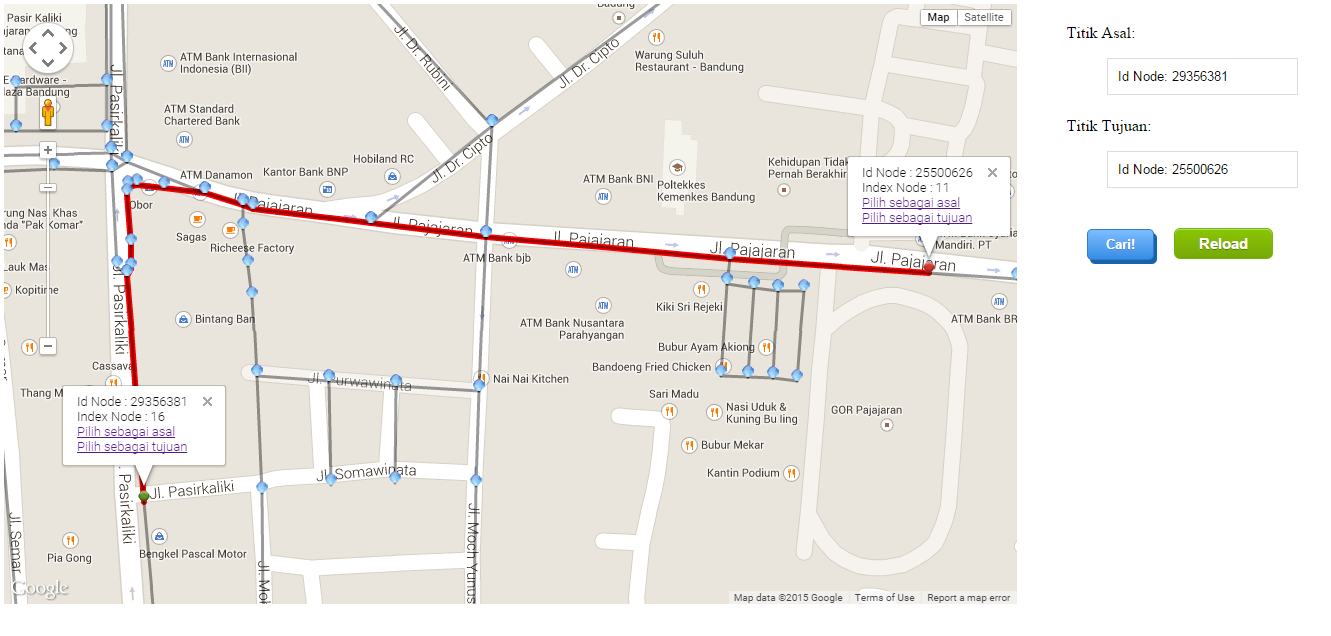
\includegraphics[scale=0.45]{Gambar/pu_visualrute}
\caption[Pengujian Visualisasi Rute Terdekat]{Pengujian Visualisasi Rute
Terdekat}
\label{fig:pu_visualrute}
\end{figure} 
\end{enumerate}

\subsection{Pengujian Eksperimental}
Pengujian eksperimental terdiri dari dua tahap, yaitu pengujian pencarian rute
dari titik asal hingga tujuan dengan beberapa pilihan rute, sehingga dapat
dipastikan bahwa aplikasi benar-benar menunjukkan rute yang terdekat. Tahap 
kedua, pengujian dilakukan dengan menggunakan tiga dokumen OSMXML yang berbeda, 
hal ini dilakukan untuk menguji bahwa aplikasi tetap berjalan dengan baik 
menggunakan dokumen OSMXML yang berbeda-beda. Ketiga dokumen tersebut diberi
nama bandung1.xml, bandung2.xml, dan bandung3.xml. Ketiga dokumen tersebut dihitung 
luasnya berdasarkan informasi \textit{latitude} dan \textit{longitude} secara
manual, berikut ini adalah cakupan area dari ketiga OSMXML tersebut:
\begin{enumerate}
  \item Bandung 1 \\
  Dokumen bandung1.xml hanya meliputi sebagian kecil Kota Bandung dengan titik
  pusat di sekitar Jalan.Pajajaran. Dokumen ini memiliki luas sekitar 0,3907 km
  persegi.
  \begin{itemize}
    \item Batas Atas : -6.9044500
    
    \item Batas Bawah : -6.9076500
    
    \item Batas Kiri : 107.5961800
    
    \item Batas Kanan : 107.6016300
  \end{itemize}

  \item Bandung 2 \\
  Dokumen bandung2.xml memiliki ukuran yang lebih besar dibandingkan dengan
  bandung1.xml, yaitu dengan luas sekitar 3,423 km persegi.
  \begin{itemize}
    \item Batas Atas : -6.9003000
    
    \item Batas Bawah : -6.9131000
    
    \item Batas Kiri : 107.5931000
    
    \item Batas Kanan : 107.6149000
  \end{itemize}
  
  \item Bandung 3 \\
  Dokumen bandung3.xml memiliki ukuran yang paling besar dan mencakup seluruh
  wilayah Kota Bandung dengan luas sekitar 415,8616 km persegi.
  \begin{itemize}
    \item Batas Atas : -6.8194
    
    \item Batas Bawah : -6.9959
    
    \item Batas Kiri : 107.553
    
    \item Batas Kanan : 107.745
  \end{itemize}
\end{enumerate}

\setcounter{secnumdepth}{3}
\setcounter{tocdepth}{3}
\subsubsection{Pengujian Rute Terdekat}
Pada bagian ini dijelaskan pengujian yang dilakukan untuk memastikan bahwa rute
yang ditunjukkan oleh aplikasi adalah rute yang paling dekat. Pengujian
dilakukan dengan memilih titik asal yang memiliki beberapa rute untuk dapat
sampai ke titik tujuan. Dipilih titik asal pada sekitar Jl. Pasirkaliki dan
titik tujuan di sekitar Jl. Dr Rum. Untuk mencapai titik tujuan terdapat
beberapa rute, di antaranya melalui Jl. Dr Rajiman, Jl. Dr Rum dan Jl. Dr Cipto.
Pada peta, dapat dilihat bahwa rute yang terdekat adalah melalui Jl. Dr Cipto dan aplikasi
juga menunjukkan rute yang sama, hasil pengujian yang dilakukan dapat dilihat
pada Gambar \ref{fig:pu_terdekat}.
\begin{figure}[h]
\centering
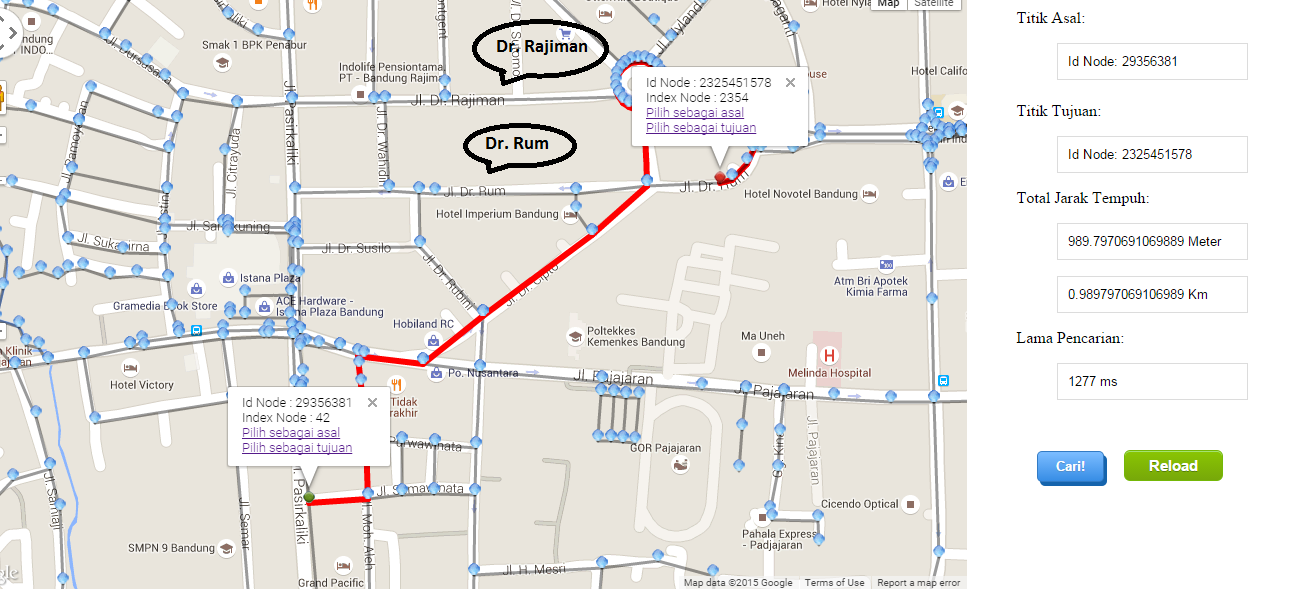
\includegraphics[scale=0.45]{Gambar/pu_terdekat}
\caption[Pengujian Rute Terdekat]{Pengujian Rute Terdekat}
\label{fig:pu_terdekat}
\end{figure}

\subsubsection{Pengujian Eksperimental Bandung 1}
Pengujian dilakukan dengan melihat waktu \textit{load} ``bandung1.xml''
(ukuran \textit{file} sebesar 98Kb), hasil pengujian dapat dilihat pada Gambar
\ref{fig:pu_bandung1}.
Pada Gambar \ref{fig:pu_bandung1} menunjukkan total waktu yang dibutuhkan untuk 
melakukan \textit{load} ``bandung1.xml'' adalah 7,710ms. Berikut ini
adalah aplikasi yang menggunakan dokumen ``bandung1.xml'' dapat dilihat pada
Gambar \ref{fig:bandung1_load}.
\begin{figure}[h]
\centering
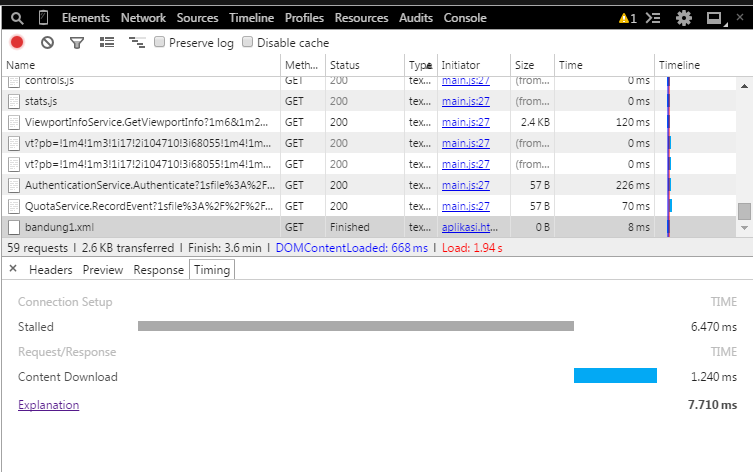
\includegraphics[scale=0.75]{Gambar/pu_bandung1}
\caption[Pengujian Bandung 1]{Pengujian Bandung 1}
\label{fig:pu_bandung1}
\end{figure}
\begin{figure}[h]
\centering
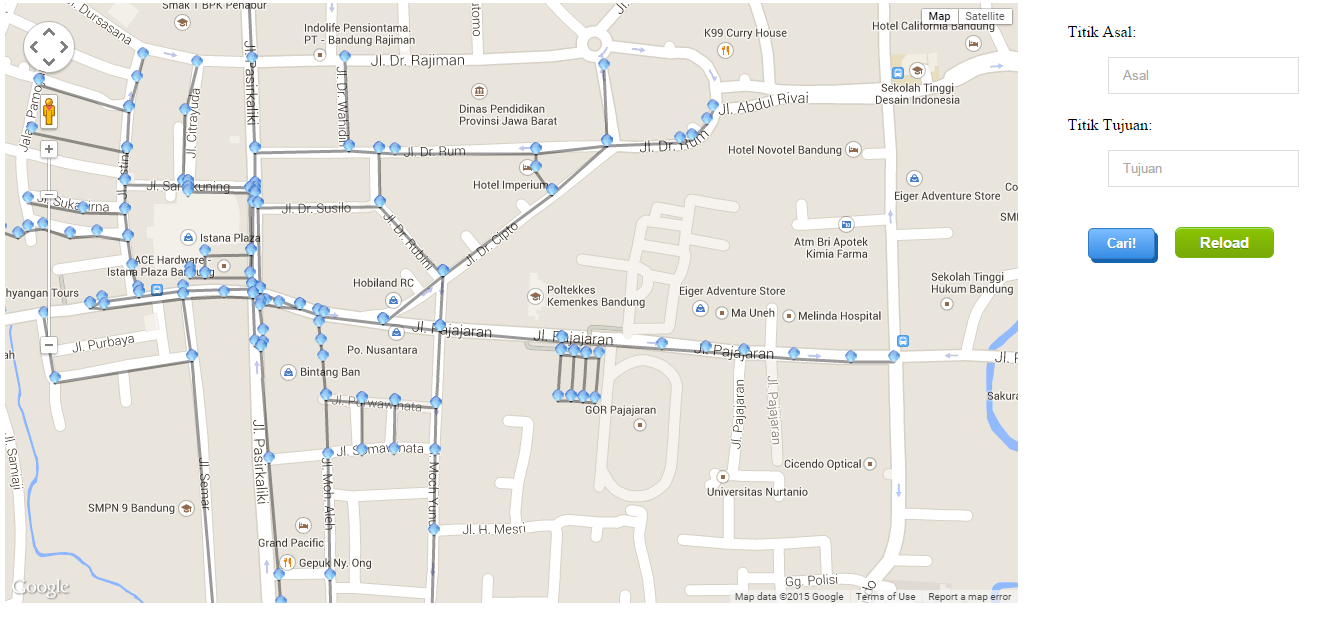
\includegraphics[scale=0.45]{Gambar/bandung1_load}
\caption[Pengujian Bandung 1]{Pengujian Bandung 1}
\label{fig:bandung1_load}
\end{figure}
\clearpage
Setelah melakukan \textit{load} aplikasi menggunakan ``bandung1.xml'', pengujian
dilanjutkan dengan mencari rute terdekat dari titik asal (Id Node : 25433686,
Index Node : 192) ke titik tujuan (Id Node : 2325451571, Index Node : 198).
\begin{figure}[h]
\centering
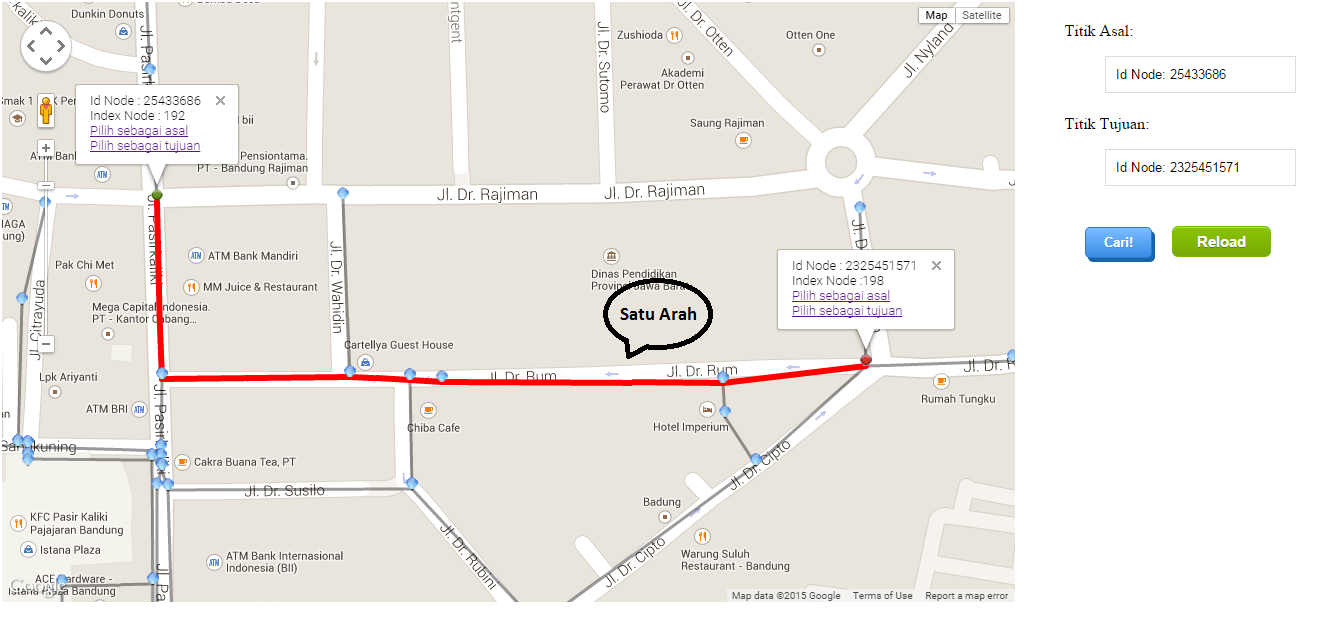
\includegraphics[scale=0.45]{Gambar/pu_bandung1_rute}
\caption[Pengujian Bandung 1]{Pengujian Bandung 1}
\label{fig:pu_bandung1_rute}
\end{figure}
Pada Gambar \ref{fig:pu_bandung1_rute} ditemukan kesalahan yaitu aplikasi
menunjukkan rute terdekat (dalam kasus pengujian melalui Jl. Dr Rum) walaupun
rute tersebut melawan arah (pada peta Google Maps menunjukkan bahwa Jl. Dr Rum
adalah jalan satu arah). Setelah dilakukan penelitian lebih lanjut, ternyata kesalahan
ditemukan pada dokumen OSMXML yaitu ``bandung1.xml'' yang tidak memberikan
informasi ``oneway'', sehingga aplikasi memasukkan informasi yang salah tersebut
ke dalam graf sebagai jalan dua arah. Berikut ini adalah potongan dokumen
``bandung1.xml'' yang memberikan informasi Jl. Dr Rum, dapat dilihat pada Gambar
\ref{fig:bandung1_xml} 
\begin{figure}[h]
\centering
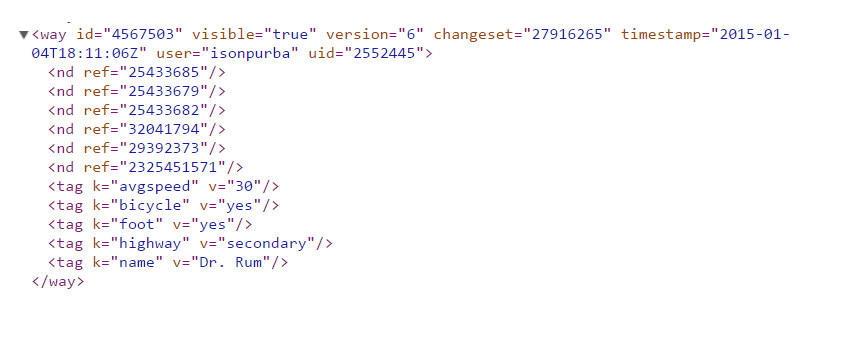
\includegraphics[scale=0.7]{Gambar/bandung1_xml}
\caption[bandung1.xml]{bandung1.xml}
\label{fig:bandung1_xml}
\end{figure}

\subsubsection{Pengujian Eksperimental Bandung 2}
Pengujian dilakukan dengan melihat waktu \textit{load} ``bandung2.xml'' (ukuran
\textit{file} sebesar 821Kb), hasil pengujian dapat dilihat pada Gambar
\ref{fig:pu_bandung2}. Pada Gambar \ref{fig:pu_bandung2} menunjukkan total waktu yang dibutuhkan untuk 
melakukan \textit{load} ``bandung2.xml'' adalah 70,460ms. 
\begin{figure}[h]
\centering
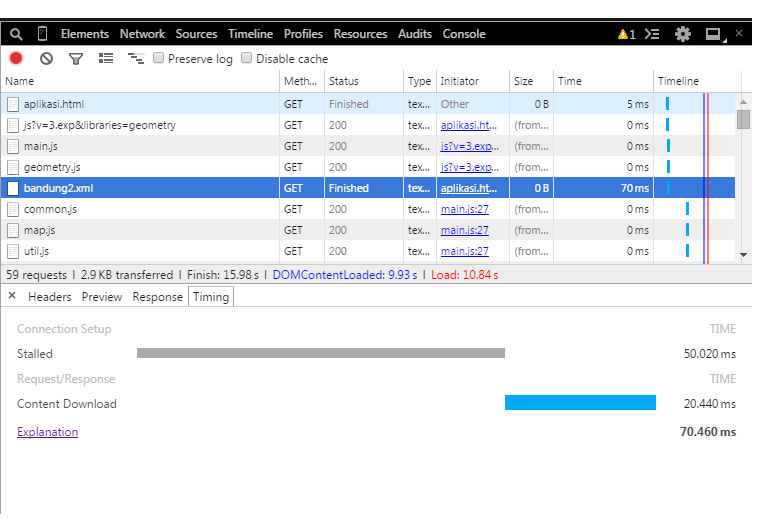
\includegraphics[scale=0.68]{Gambar/pu_bandung2}
\caption[Pengujian Bandung 2]{Pengujian Bandung 2}
\label{fig:pu_bandung2}
\end{figure}
\begin{figure}[h]
\centering
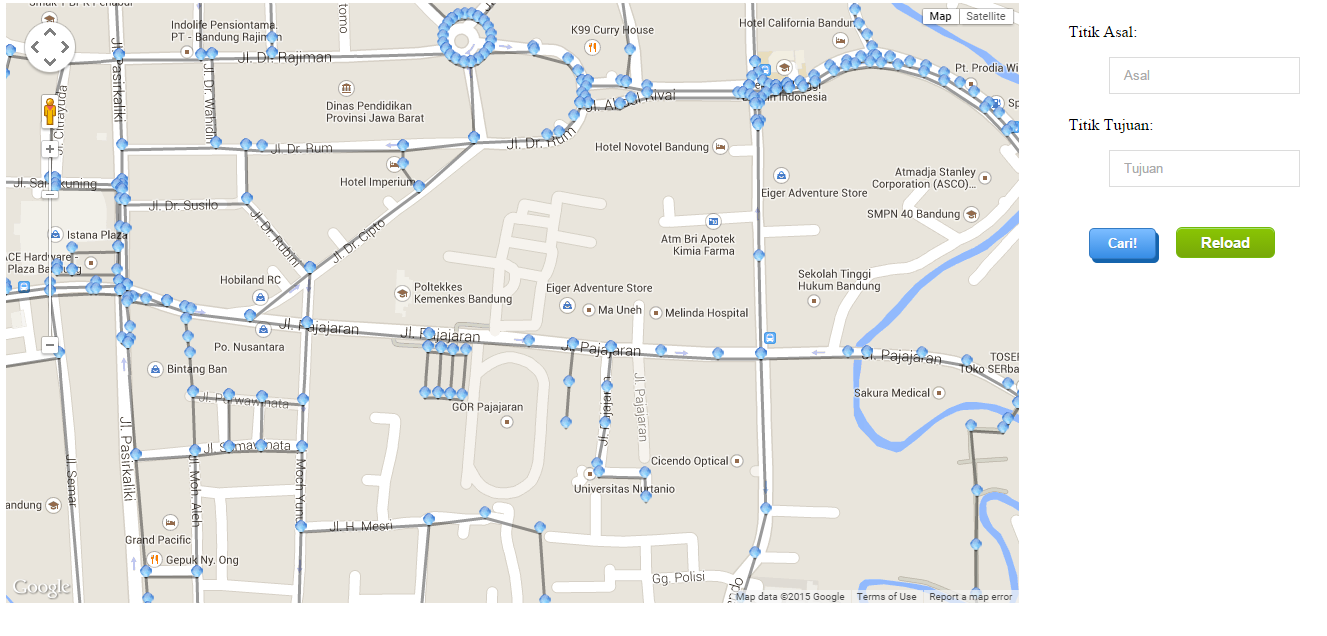
\includegraphics[scale=0.43]{Gambar/bandung2_load}
\caption[Pengujian Bandung 2]{Pengujian Bandung 2}
\label{fig:bandung2_load}
\end{figure}
\clearpage
Berikut ini adalah aplikasi yang menggunakan dokumen ``bandung2.xml'' dapat
dilihat pada Gambar \ref{fig:bandung2_load}.
Setelah melakukan \textit{load} aplikasi menggunakan ``bandung2.xml'', pengujian
dilanjutkan dengan mencari rute terdekat dari titik asal (Id Node : 29356503,
Index Node : 47) ke titik tujuan (Id Node : 1700554920, Index Node : 1163).
Hasil pengujian dapat dilihat pada Gambar \ref{fig:pu_bandung2_rute}.
\begin{figure}[h]
\centering
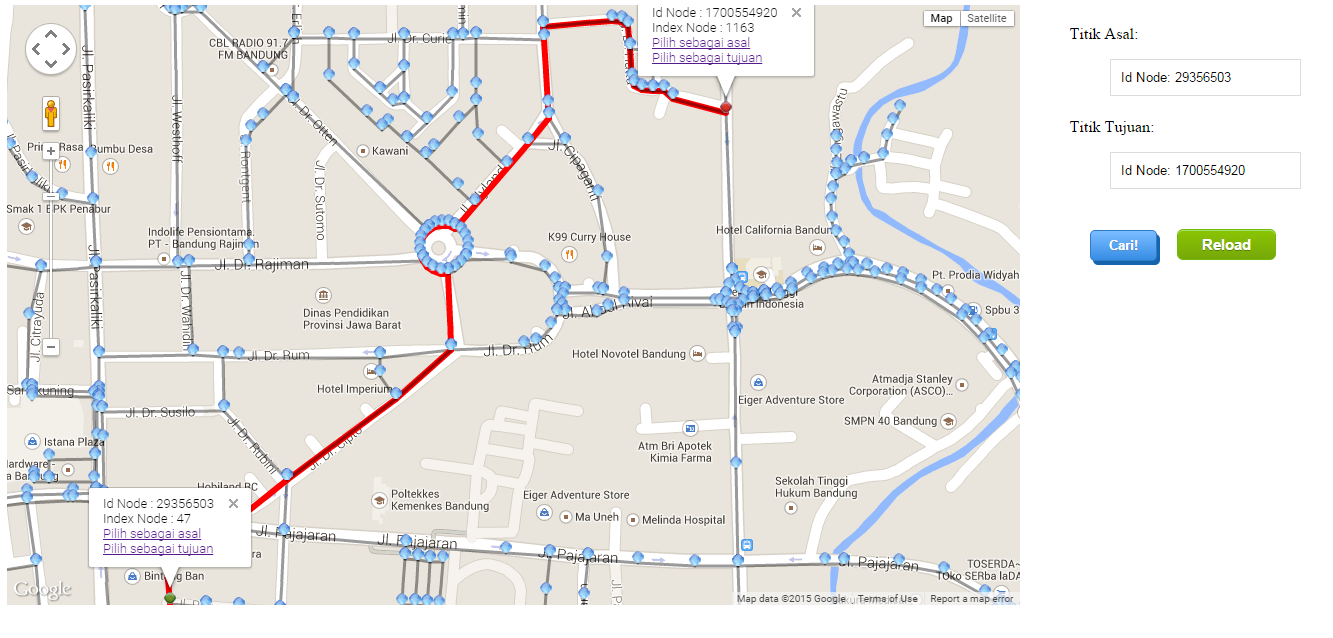
\includegraphics[scale=0.45]{Gambar/pu_bandung2_rute}
\caption[Pengujian Bandung 2]{Pengujian Bandung 2}
\label{fig:pu_bandung2_rute}
\end{figure}

\subsubsection{Pengujian Eksperimental Bandung 3}
Pengujian dilakukan dengan melihat waktu \textit{load} ``bandung3.xml'' (ukuran
\textit{file} sebesar 17.631Kb). Dokumen ``bandung3.xml'' adalah OSMXML yang
mencakup seluruh wilayah Kota Bandung, berdasarkan pengujian yang telah dilakukan, 
aplikasi tidak berhasil untuk menggunakan ``bandung3.xml''. Hal ini disebabkan oleh 
dokumen ``bandung3.xml'' yang terlalu besar dan waktu \textit{load} yang terlalu
lama.

\subsubsection{Hasil Pengujian}
Berdasarkan pengujian eksperimental yang telah dilakukan, diketahui beberapa hal
yaitu:
\begin{enumerate}
  \item Aplikasi telah menunjukkan rute yang benar-benar terdekat.
  
  \item \textit{Load} dokumen OSMXML\\
  Hasil pengujian ketiga dokumen OSMXML dapat dilihat pada Tabel
  \ref{tab:doc_xml}.
\begin{table}[h]
\centering
\caption{Dokumen OSMXML} 
\label{tab:doc_xml}
\begin{tabular}{|c|c|c|c|c|}
\hline
          & Ukuran File & Waktu Load & Jumlah Node & Jumlah Edge \\ \hline
Bandung 1 & 98 Kb       & 7,710 ms   & 125         & 141         \\ \hline
Bandung 2 & 821 Kb      & 70,460 ms  & 955        & 1073        \\ \hline
Bandung 3 & 17.631 Kb   & -          & -           & -           \\ \hline
\end{tabular}
\end{table}

  Berdasarkan pengujian tersebut, ``bandung3.xml" tidak berhasil dibuka
  karena ukurannya yang terlalu besar dan diketahui bahwa semakin besar dokumen
  OSMXML, semakin besar pula waktu \textit{load} yang diperlukan.
  
  \item Kesalahan\\
  Kesalahan ditemukan ketika pengujian berlangsung, yaitu rute terdekat yang
  ditunjukkan oleh aplikasi melawan arus jalan, hal ini disebabkan oleh dokumen
  OSMXML yang tidak memberikan informasi ``oneway''.
\end{enumerate}











